\section{Bayes' Theorem}


\begin{frame}[c]{Bayes'sche Theorem: xkcd}
    \begin{multicols}{2}
    \begin{itemize}
        \item[]<1> 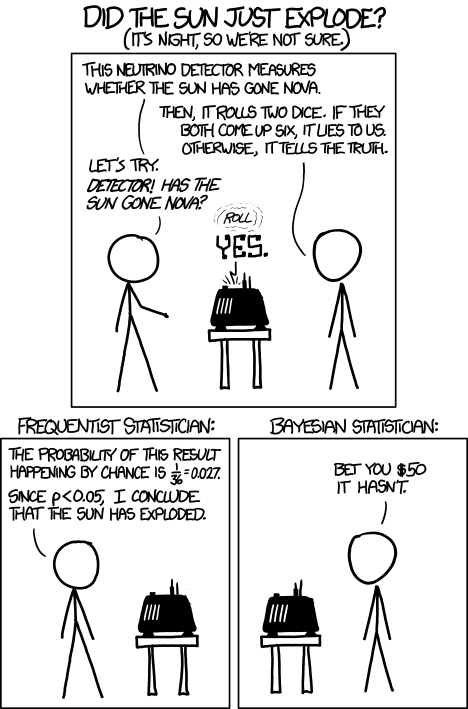
\includegraphics[height=7cm]{strategy/xkcd_frequentists_vs_bayesians.png}
        \item[]<2> 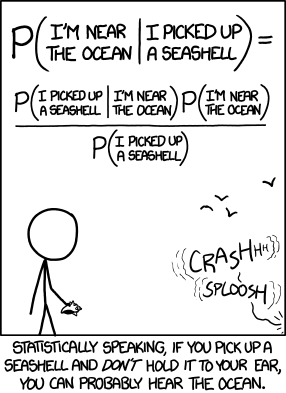
\includegraphics[height=7cm]{strategy/xkcd_seashell.png}
    \end{itemize}
    \end{multicols}
\end{frame}


\begin{frame}[c]{Das Bayes'sche Theorem}
    \Large
    \[
        P(A|X) = \frac{P(X|A) * P(A)}{P(X|A) * P(A) + P(X|\neg A) * P(\neg A)}
    \]
\end{frame}


\begin{frame}[c]{Bayes vs Klassische Stastik}
    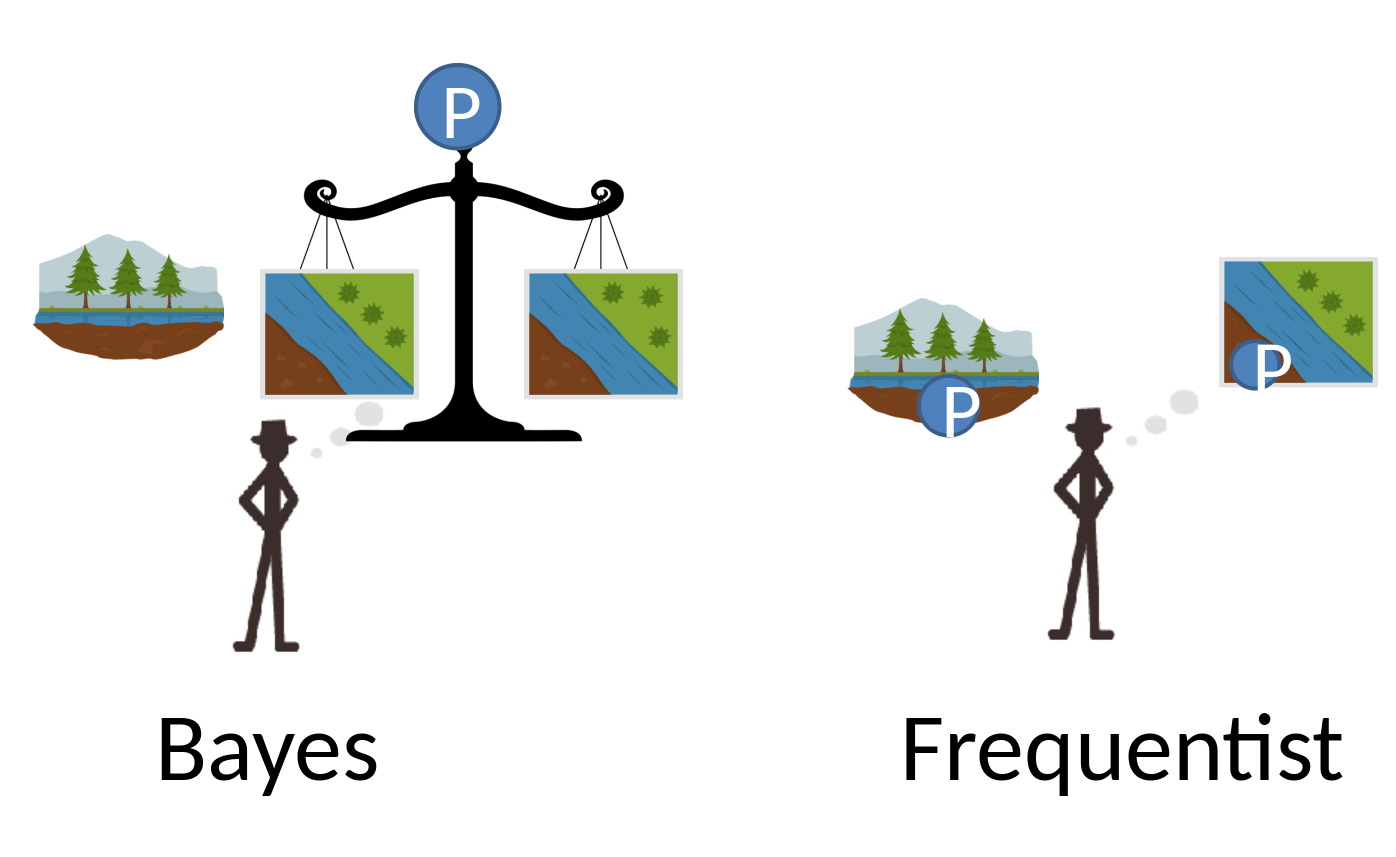
\includegraphics[width=\textwidth]{bayes_vs_freq}
\end{frame}



